
%(BEGIN_QUESTION)
% Copyright 2010, Tony R. Kuphaldt, released under the Creative Commons Attribution License (v 1.0)
% This means you may do almost anything with this work of mine, so long as you give me proper credit

Gasoline and diesel engines differ in their thermodynamic cycles.  The Force/Stroke graphs of each engine type are shown here for comparison:

$$\includegraphics[width=15.5cm]{i04433x01.eps}$$

The prolonged ignition cycle of the diesel cycle is a consequence of how diesel fuel burns when it is injected into the hot, compressed air inside the cylinder: it burns in stages rather than all at once as is the case with a gasoline engine where the entire cylinder's volume is filled with an optimal mix of fuel and air.

Assuming all other factors are equal, which type of engine will deliver more net energy per cycle?  Explain your reasoning.

\underbar{file i04433}
%(END_QUESTION)





%(BEGIN_ANSWER)

The diesel cycle delivers more net energy: although the energy ``invested'' in the compression stroke is the same for both engines in this example, the diesel's power stroke constitutes a greater amount of energy because the area under the power curve is greater (owing to the prolonged ignition cycle).

\vskip 10pt

This is the main reason why diesel engines are so much more efficient than gasoline engines, all other factors being equal.

%(END_ANSWER)





%(BEGIN_NOTES)


%INDEX% Mathematics, calculus: integral (work)
%INDEX% Mathematics, calculus: integration (numerical)
%INDEX% Process: engine P-V curves

%(END_NOTES)


